\documentclass[10pt]{article}

\usepackage{geometry}

\geometry{a4paper, left=20mm, right=20mm, bottom=20mm, top=20mm}

\usepackage[english]{babel}
\usepackage[utf8]{inputenc}
\usepackage{amsmath}
\usepackage{dsfont}
\usepackage[most]{tcolorbox}
\usepackage{varwidth}
\usepackage{graphicx}
\usepackage{subcaption}

\usepackage[T1]{fontenc}
\usepackage[sfdefault]{roboto}
\usepackage{roboto-mono}
\usepackage{fontawesome5}

\usepackage{listings}
\usepackage{listingsutf8}
\usepackage{xcolor}

\lstset{
    inputencoding=utf8/latin1,
    backgroundcolor=\color{gray!10},
    frame=single,
    numberstyle=\tiny,
}

\lstdefinestyle{patch}{
    language={},
    breaklines=true,
    basicstyle=\ttfamily,
    keywordstyle=\color{blue},
    commentstyle=\color{gray},
    morecomment=[f][\color{red}]{-},
    morecomment=[f][\color{olive}]{+},
    captionpos=b,
    numbers=left,
}

\lstdefinestyle{go}{
    inputencoding=utf8,
    extendedchars=true,
    literate={і}{{i}}1,
    keywords={break, case, chan, const, continue, default, defer, else, fallthrough,
        for, func, go, goto, if, import, interface, map, package, range, return,
        select, struct, switch, type, var, bool, byte, complex64, complex128,
        float32, float64, int8, int16, int32, int64, string, uint8, uint16, uint32, uint64, int, uint, uintptr, error},
    keywordstyle=\color{blue}\bfseries,
    ndkeywords={true, false, iota, nil},
    ndkeywordstyle=\color{red}\bfseries,
    identifierstyle=\color{black},
    sensitive=true,
    comment=[l]{//},
    morecomment=[s]{/*}{*/},
    commentstyle=\color{green}\ttfamily,
    stringstyle=\color{orange}\ttfamily,
    morestring=[b]',
    morestring=[b]",
    tabsize=2,
    showspaces=false,
    showtabs=false,
    keepspaces=true,
    columns=flexible,
    showstringspaces=false,
    breaklines=true,
    breakatwhitespace=true,
    basicstyle=\ttfamily,
    captionpos=b,
    numbers=left,
}

\lstdefinestyle{python}{
    basicstyle=\ttfamily\small,
    keywordstyle=\color{blue},
    stringstyle=\color{red},
    commentstyle=\color{green!60!black},
    morecomment=[l][\color{magenta}]{\#},
    showstringspaces=false,
    tabsize=4,
    breaklines=true,
    captionpos=b,
    numbers=left,
}

\lstdefinestyle{bash}{
    basicstyle=\ttfamily\small,
    keywordstyle=\color{blue},
    stringstyle=\color{red},
    commentstyle=\color{green!60!black},
    morekeywords={sudo, cd, ls, echo, export, source, mv, cp, rm, mkdir, chmod, chown},
    showstringspaces=false,
    tabsize=4,
    breaklines=true,
    captionpos=b,
    numbers=left,
}

\usepackage{hyperref}

\hypersetup{
    colorlinks=true,
    linkcolor=black,
    filecolor=black,
    urlcolor=cyan,
}

\setlength\parindent{0pt}

\newcommand{\definition}[2]{
\begin{tcolorbox}[
		title={#1},hbox,
		colframe=green!75!black,
		colback=green!40!white,
		coltitle=black,
	]
    \begin{varwidth}{\textwidth}
		#2
    \end{varwidth}
\end{tcolorbox}
}

\makeatletter
\renewcommand*\env@matrix[1][\arraystretch]{%
  \edef\arraystretch{#1}%
  \hskip -\arraycolsep
  \let\@ifnextchar\new@ifnextchar
  \array{*\c@MaxMatrixCols c}}
\makeatother

\title{Replme Documentation}
\author{Jacob Bachmann}
\date{ }

\begin{document}

\maketitle

\tableofcontents

\section{Overview}

\begin{figure}
	\centering
	\begin{subfigure}{0.478\textwidth}
		\centering
		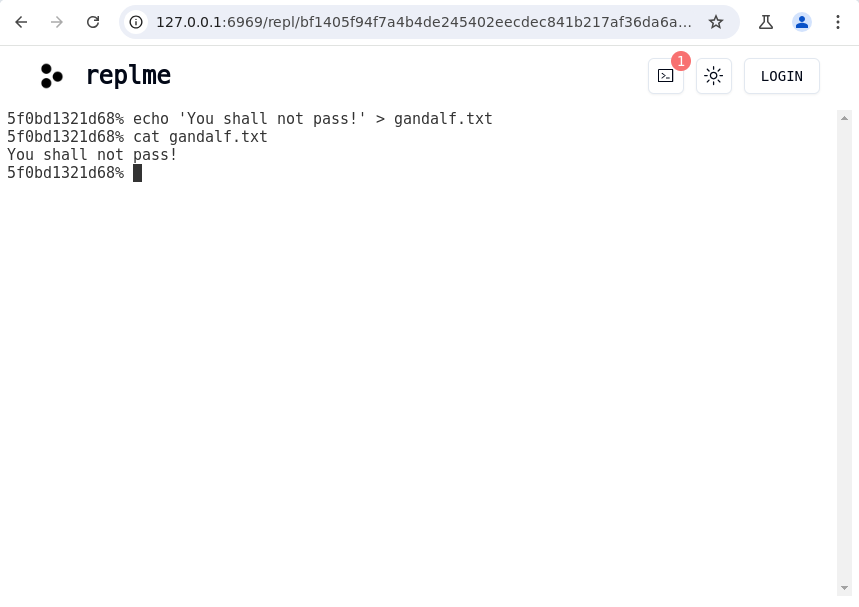
\includegraphics[width = \textwidth]{src/repl}
		\caption{REPL}
	\end{subfigure}
	\begin{subfigure}{0.49\textwidth}
		\centering
		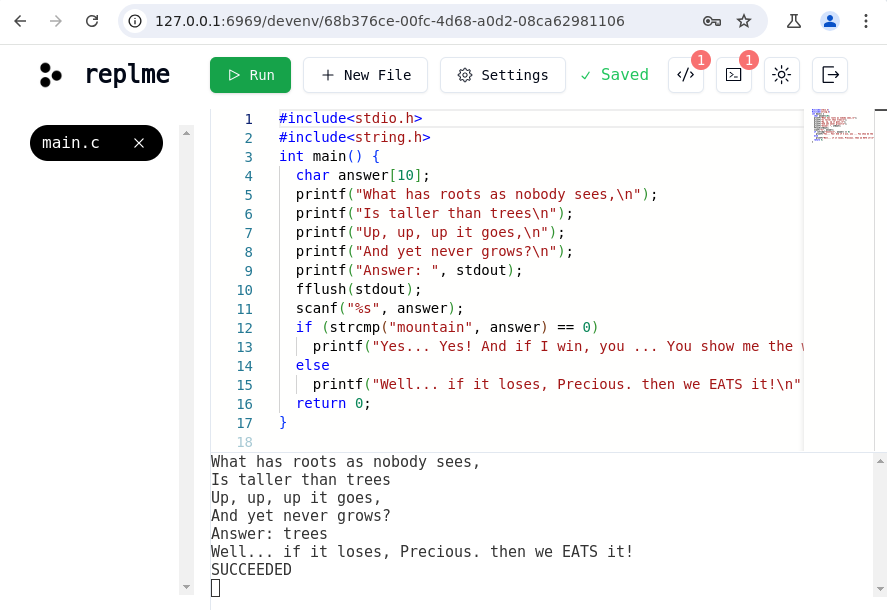
\includegraphics[width = \textwidth]{src/devenv}
		\caption{DEVENV}
	\end{subfigure}
\end{figure}

\robotomonoRegular{replme} provides users with the possibility to create development environments (DEVENVs) and spawn "throw-away" shells (REPLs) in the browser. It is strongly influenced by \href{https://replit.com}{replit.com}. \\

The infrastructure consists of a nginx reverse-proxy that forwards all requests to the Next.js frontend server, except for requests whose path starts with \robotomonoRegular{/api} -- those are forwarded to the golang+gin backend (hereafter MAIN-BACKEND). The MAIN-BACKEND persist data in a PostgreSQL instance. \\

To spawn a REPL or compile code in a DEVENV the MAIN-BACKEND interfaces with a docker-in-docker instance (DIND) to create Alpine Linux containers (hereafter ALPINEs). The IO of the command running on the aplines is proxied to the web client by the MAIN-BACKEND. \\

The ALPINEs themselves have another golang+gin backend running on them (hereafter CHILD-BACKEND). The MAIN-BACKEND interfaces with the CHILD-BACKEND to create/authenticate users and spawn commands on the ALPINEs.

\section{Directory Structure}

\lstinputlisting[]{src/dir-structure.txt}

\section{Vulnerability \#1 -- CRC}

\subsection{How it works}

REPLs are \robotomonoRegular{/bin/zsh} shells in the user land of a temporary ALPINE environment. Their filesystem is persisted for a limited time. When a REPL is spawned, the client generates a random pair of 60 bytes username and password, and sends the pair to the MAIN-BACKEND. The MAIN-BACKEND stores the pair in the user session and spawns an ALPINE. The identifier of the ALPINE is the CRC checksum of the random 60 bytes username. However, it isn't a typical CRC32 or CRC64, instead it is a CRC251 using the prime polynomial of degree 251:
\begin{center}
	\robotomonoRegular{0x8561cc4ee956c6503c5da0ffacb20feabb3eb142e7645e7ff1a2067fd8e1cfb}
\end{center}

Herein lies the first vulnerability. CRC is no cryptographically secure hashing function. Given a target username $a$, the goal is to find a second pre-image $a'$ such that $\texttt{CRC251}(a) = \texttt{CRC251}(a')$. With $a'$, the adversary gets access to the ALPINE created for $a$, including read-only access on \robotomonoRegular{/home/<username>} where the flag is stored. \\

\begin{center}
	\definition{CRC}{
	\textit{Let $a, p \in \mathds{F}_2[x]$ then there are unique polynomial $b, r \in \mathds{f}_2[x]$ \\ with $deg(r) < deg(p)$ such that}
	\begin{equation*}
		a(x) = b(x) \cdot p(x) + r(x)
	\end{equation*}
	\textit{where $a(x)$ is the message polynomial (input), $p(x)$ the \\ generator polynomial, $b(x)$ the quotient polynomial, \\ and $r(x)$ the remainder polynomial (CRC).}
	}
\end{center}

\vspace*{.4cm}
Hence, to calculate the CRC: $r(x) = a(x)\bmod p(x)$. Intuitively, finding a second pre-image under these conditions is easy. Calculate a delta $\Delta(x) = b_\Delta(x) \cdot\ p(x)$ and add it to the given username:
\begin{equation}
	a'(x) = a(x) + \Delta(x) = a(x) + b_\Delta(x)p(x) = a(x) + 0 = a(x) = r(x) \bmod p(x)
\end{equation}

But what kind of polynomial yields our data (e.g. username)? All bits in our data's bit-representation are elements from $\mathds{F}_2$ with addition ($\oplus$ on bits) and multiplication ($\odot$ on bits). Therefore, the polynomial for data bits $a=a_{l-1}...a_0$ looks like this:

\begin{equation}
	a(x) = a_{l-1}x^{l-1}+a_{l-2}x^{l-2}+..+a_1x+a_0
\end{equation}

\vspace*{.4cm}
Note, for technical reasons $a(x)$ is multiplied with $x^{deg(p)}$, or $<< deg(p)$ on bits. \\

Back in context of replme, the MAIN-BACKEND only allows ASCII characters \robotomonoRegular{a-z} and \robotomonoRegular{0-5} for usernames. Before calculating the checksum, the characters are mapped the following way:
\begin{equation}
	\label{eq:char-mapping}
	\begin{tabular}{l l l l l}
		0       & $\Rightarrow$ & \`\                     & GRAVE ACCENT  & $\robotomonoRegular{01100000}_2$ \\
		a       & $\Rightarrow$ & a                       &               & $\robotomonoRegular{01100001}_2$ \\
		$\dots$ &               & $\dots$                 &               & $\dots$                          \\
		z       & $\Rightarrow$ & z                       &               & $\robotomonoRegular{01111010}_2$ \\
		1       & $\Rightarrow$ & \{                      & OPENING BRACE & $\robotomonoRegular{01111011}_2$ \\
		2       & $\Rightarrow$ & |                       & VERTICAL BAR  & $\robotomonoRegular{01111100}_2$ \\
		3       & $\Rightarrow$ & \}                      & CLOSING BRACE & $\robotomonoRegular{01111101}_2$ \\
		4       & $\Rightarrow$ & \~{}                    & TILDE         & $\robotomonoRegular{01111110}_2$ \\
		5       & $\Rightarrow$ & \robotomonoRegular{DEL} & DELETE        & $\robotomonoRegular{01111111}_2$
	\end{tabular}
\end{equation}

We can see that the bit representation of the set of the mapped allowed characters follows the pattern\\ $\robotomonoRegular{011*****}_2$. \\

This restriction also aplies to $a'$. Under this condition it is not anymore trivial to find some $\Delta$, since it must have the bit representation $\robotomonoRegular{000*****...000*****}_2$, such that:
\begin{equation}
	% \arraycolsep=1.4pt
	\def\arraystretch{1.2}
	\begin{array}{lll}
		       & \robotomonoRegular{011*****...011***** 0...0}_2 & \color{gray}(a)      \\
		\oplus & \robotomonoRegular{000*****...000***** 0...0}_2 & \color{gray}(\Delta) \\
		=      & \robotomonoRegular{011*****...011***** 0...0}_2 & \color{gray}(a')     \\
	\end{array}
\end{equation}

For the in replme given polynomial of degree 251 and usernames of length 60 bytes, this leaves us with the equation:
\begin{equation*}
	\underbrace{(\robotomonoRegular{000*****...000*****}_2)}_{\texttt{60 times}} << {251} = b_\Delta\cdot p
\end{equation*}
or more specific:

\begin{equation}
	\underbrace{\sum_{i=0}^{59}\left(\sum_{j=0}^{4}*x^{8*i+j+251}+\sum_{k=5}^{7}0x^{8*i+k+251}\right)+\sum_{l=0}^{250}0x^l}_{\Delta(x)} = \underbrace{\left(\sum_{m=0}^{59*8+7}b_mx^m\right)}_{b_\Delta(x)} \cdot \underbrace{\left(\sum_{n=0}^{251}p_nx^n\right)}_{p(x)}
\end{equation}

Now, we can multiply $b_\Delta(x)\cdot p(x)$, do a coefficient comparison with $\Delta(x)$ where the coefficients are $0$, and create an underdetermined equation system: $Ab=0$. The kernel of the matrix $A$ spans the set of all $b_\Delta$ that -- multiplied with $p$ -- give us all possible $\Delta$ that (for any given input $a$ of length 60 bytes) added to input $a$ give us all second pre images (of length 60 bytes). \\

\subsection{Example}

Let's find the $\Delta$'s for the polynomial \robotomonoRegular{0x14} of degree 4 and input length of 1 byte. \\

This gives us following equations:
\begin{equation}
	\begin{aligned}
		p(x)                  & = x^4 + x^2                                                                               \\
		b_\Delta(x)           & = b_7x^7 + b_6x^6 + b_5x^5 + b_4x^4 + b_3x^3 + b_2x^2 + b_1x^1 + b_0x^0                   \\
		b_\Delta(x)\cdot p(x) & = b_7x^{11} + b_6x^{10} + b_7x^{9} + b_5x^{9} + b_6x^{8} + b_4x^{8} + b_5x^{7} + b_3x^{7} \\
		                      & + b_4x^{6} + b_2x^{6} + b_3x^{5} + b_1x^{5} +b_2x^{4} + b_0x^{4} + b_1x^{3} + b_0x^2      \\
		\Delta(x)             & = 0x^{11} + 0x^{10} + 0x^{9} + *x^{8} + *x^{7} + *x^{6} + *x^{5} + *x^{4}                 \\
		                      & + 0x^{3} + 0x^{2} + 0x^{1} + 0x^{0}
	\end{aligned}
\end{equation}

Now we do a coefficient comparison of $b_\Delta(x)\cdot p(x)$ with $\Delta(x)$ for the powers of $x$ where the coefficient is $0$ in $\Delta(x)$. This resultings in the equation $Ab=0$:
\begin{equation}
	\begin{aligned}
		 & \ \ \ \color{gray}\begin{matrix}
			                     b_0 & \!\! b_1 & \!\! b_2 & \!\! b_3 & \!\! b_4 & \!\! b_5 & \!\! b_6 & \!\! b_7
		                     \end{matrix} \\
		\color{gray}\begin{matrix}[1.15]
			            x^{11} \\ x^{10} \\ x^9 \\ x^3 \\ x^2 \\ x^1 \\ x^0
		            \end{matrix}
		 & \begin{pmatrix}
			   0 & 0 & 0 & 0 & 0 & 0 & 0 & 1 \\
			   0 & 0 & 0 & 0 & 0 & 0 & 1 & 0 \\
			   0 & 0 & 0 & 0 & 0 & 1 & 0 & 1 \\
			   1 & 0 & 1 & 0 & 0 & 0 & 0 & 0 \\
			   0 & 1 & 0 & 0 & 0 & 0 & 0 & 0 \\
			   1 & 0 & 0 & 0 & 0 & 0 & 0 & 0 \\
			   0 & 0 & 0 & 0 & 0 & 0 & 0 & 0 \\
			   0 & 0 & 0 & 0 & 0 & 0 & 0 & 0
		   \end{pmatrix}
		\begin{pmatrix}
			b_0 \\ b_1 \\ b_2 \\ b_3 \\ b_4 \\ b_5 \\ b_6 \\ b_7
		\end{pmatrix} =
		\begin{pmatrix}
			0 \\ 0 \\ 0 \\ 0 \\ 0 \\ 0 \\ 0 \\ 0
		\end{pmatrix}
	\end{aligned}
\end{equation}

To solve that underdetermined system we can just calculate the kernel $\ker(A)$, with following result:
\begin{equation}
	\begin{aligned}
		             & \ \ \ \ \ \ \color{gray}\begin{matrix}
			                                       b_0 & \!\! b_1 & \!\! b_2 & \!\! b_3 & \!\! b_4 & \!\! b_5 & \!\! b_6 & \!\! b_7
		                                       \end{matrix} \\
		b_{\Delta_1} & = \begin{pmatrix}
			                 0 & 0 & 0 & 1 & 0 & 0 & 0 & 0
		                 \end{pmatrix}                                                                          \\
		b_{\Delta_2} & = \begin{pmatrix}
			                 0 & 0 & 0 & 0 & 1 & 0 & 0 & 0
		                 \end{pmatrix}
	\end{aligned}
\end{equation}

Each combination of the elements in the kernel gives us a valid $b_\Delta$. Let's calculate the $\Delta$:
\begin{equation}
	% \arraycolsep=1.4pt
	\def\arraystretch{1.3}
	\begin{array}{rlll}
		\color{gray} \emptyset:                 & \Delta_0(x)  = & 0 \cdot p(x)         & = 0                     \\
		\color{gray} b_{\Delta_1}:              & \Delta_1(x)  = & x^3 \cdot p(x)       & = x^7 + x^5             \\
		\color{gray} b_{\Delta_2}:              & \Delta_2(x)  = & x^4 \cdot p(x)       & = x^8 + x^6             \\
		\color{gray} b_{\Delta_1}+b_{\Delta_2}: & \Delta_3(x)  = & (x^4+x^3) \cdot p(x) & = x^8 + x^7 + x^6 + x^5
	\end{array}
\end{equation}

Let's calculate the pre-images of $\texttt{CRC4}(\texttt{"s"}) = \texttt{CRC4}(\robotomonoRegular{01110011}_2$):
	\begin{equation}
		% \arraycolsep=1.4pt
		\def\arraystretch{1.3}
		\begin{array}{lll}
			a'_0  = \texttt{"s"} << 4 \oplus \Delta_0 = \robotomonoRegular{011100110000}_2 \oplus\robotomonoRegular{000000000000}_2 = \robotomonoRegular{011100110000}_2 = \texttt{"s"} << 4 \\
			a'_1  = \texttt{"s"} << 4 \oplus \Delta_1 = \robotomonoRegular{011100110000}_2 \oplus\robotomonoRegular{000010100000}_2 = \robotomonoRegular{011110010000}_2 = \texttt{"y"} << 4 \\
			a'_2  = \texttt{"s"} << 4 \oplus \Delta_2 = \robotomonoRegular{011100110000}_2 \oplus\robotomonoRegular{000101000000}_2 = \robotomonoRegular{011001110000}_2 = \texttt{"g"} << 4 \\
			a'_3  = \texttt{"s"} << 4 \oplus \Delta_3 = \robotomonoRegular{011100110000}_2 \oplus\robotomonoRegular{000111100000}_2 = \robotomonoRegular{011011010000}_2 = \texttt{"m"} << 4 \\
		\end{array}
	\end{equation}

	Therefore, \texttt{"s"}, \texttt{"y"}, \texttt{"g"}, and \texttt{"m"} are pre-images for $\texttt{CRC4}(\texttt{"s"})$.

	\subsection{Exploit}

	In case of our polynomial, the kernel has $48$ base vectors that span a total of $2^{48}=281474976710656$ elements ($b_\Delta$). The adversaries can choose a few random $b_\Delta$'s. Due to the large number of possible elements, collisions with other adversaries are very unlikely.

	For a by the \robotomonoRegular{attack\_info.json} given username $a$, some randomly choosen $\Delta$, and the function $map$ that maps the characters like in Table \ref{eq:char-mapping}, the steps to exploit are as follows:
\begin{enumerate}
	\item Calculate $a' = map^{-1}(map(a) \oplus (\Delta >> 251))$.
	\item Create a new REPL session: \\
	      \robotomonoRegular{POST /api/repl} \\
	      \robotomonoRegular{Request-Body: \{ "username": "<$a'$>", "password": "<somepassword>" \}} \\
	      \robotomonoRegular{Response-Body: \{ "id": "<replid>" \}}
	\item With the new session cookie and \robotomonoRegular{replid} open a websocket connection: \\
	      \robotomonoRegular{ws://<host>:<port>/api/repl/<replid>}
	\item Send the following shell command over the websocket connection: \\
	      \robotomonoRegular{echo FLAG \&\& cat ../<$a$>/flagstore.txt \&\& echo OK}
	\item Flags are Base64 encoded, therefore, match the output with the RegEx \\
	      \robotomonoRegular{FLAG\textbackslash s*([A-Za-z0-9\textbackslash +\textbackslash =\textbackslash /]+)\textbackslash s*OK} \\
	      until a match is found.
\end{enumerate}

\subsection{Fix}

The fix is a rather simple one. Replace \robotomonoRegular{CRC251} with a cryptographically secure hashing function, e.g. \robotomonoRegular{SHA224}. See Listing \ref{lst:crc} in Section \ref{sec:appendix} Appendix for the patch.

\section{Vulnerability \#2 -- Path traversal}

\subsection{How it works}

In a DEVENV the user can create, edit, delete, and execute source code. The source code files are persisted in the hosts filesystem (under \robotomonoRegular{/<prefix>/<devenvuuid>/<filename>}) and executed within ALPINEs.

To get the contents of a DEVENV file the owner can request
\begin{center}
	\robotomonoRegular{GET /api/devenv/<devenvuuid>/files/<filename>}
\end{center}
However, all \robotomonoRegular{/api/devenv/...} endpoints also accept a query parameter \robotomonoRegular{?uuid=<otheruuid>} which, when specified, overloads the \robotomonoRegular{<devenvuuid>}.

\lstinputlisting[caption=service/backend/server/router.go\ (lines\ 110-148), style=go, label={lst:devenv-uuid-snippet}]{src/devenv-uuid-snippet.go}

The extracted DEVENV and \robotomonoRegular{uuid} are saved in the current requests context. We can see, that \robotomonoRegular{id} is seemingly sanitized via \robotomonoRegular{util.ExtractUuid}. Instead of using the DEVENV from the context (that definitely belongs to the current user), the eventually executed controller function \robotomonoRegular{GetFileContent} uses the \robotomonoRegular{uuid} to compute the path of the requested file content.

\lstinputlisting[caption=service/backend/controller/devenv.go\ (lines\ 239-262), style=go, label={lst:devenv-file-content-snippet}]{src/devenv-file-content-snippet.go}

Herein lies the second vulnerability. Due to the \robotomonoRegular{util.ExtractUuid} function which does not sanitize user input correctly, the adversary is able to use path traversal to retrieve the contents of files belonging to DEVENVs owned by other users.

\lstinputlisting[caption=service/backend/util/encoding.go\ (lines\ 21-29), style=go, label={lst:extract-uuid-snippet}]{src/extract-uuid-snippet.go}

In line 6 in Listing \ref{lst:extract-uuid-snippet} the "i" of the left \robotomonoRegular{uuid} variable is not an ASCII "i". Instead it is the "Cyrillic Small Letter Byelorussian-Ukrainian I" (\robotomonoRegular{U+0456}), a unicode look-alike. Therefore, in line 8, the \robotomonoRegular{uuid} defined in line 1 which is just set to the user input is returned -- completely unescaped.

\subsection{Exploit}

For a by the \robotomonoRegular{attack\_info.json} given DEVENV's \robotomonoRegular{targetUuid}, the steps to exploit are as follows:
\begin{enumerate}
	\item Register a new random user: \\
	      \robotomonoRegular{POST /api/auth/register} \\
	      \robotomonoRegular{Request-Body \{ "username": "...", "password": "..." \}}
	\item Login with the newly created user: \\
	      \robotomonoRegular{POST /api/auth/login} \\
	      \robotomonoRegular{Request-Body \{ "username": "...", "password": "..." \}}
	\item Create some random DEVENV: \\
	      \robotomonoRegular{POST /api/devenv} \\
	      \robotomonoRegular{Request-Body \{ "name": "...", "buildCmd": "...", "runCmd": "..." \}} \\
	      \robotomonoRegular{Response-Body \{ "devenvUuid": "<ownUuid>" \}}
	\item Get the file content for \robotomonoRegular{targetUuid}: \\
	      \robotomonoRegular{GET /api/devenv/<ownUuid>/files/flagstore.txt?uuid=<ownUuid>\%2F..\%2F<targetUuid>} \\
\end{enumerate}

\subsection{Fix}

To fix this vulnerability, patch the \robotomonoRegular{GetFileContent} function in Listing \ref{lst:devenv-file-content-snippet} to use the DEVENV from the context instead of the \robotomonoRegular{uuid}. See Listing \ref{lst:path-traversal} in Section \ref{sec:appendix} Appendix for the patch.

\section{Vulnerability \#3 -- Unintended RCE}

\subsection{How it works}

All the ALPINEs share the same DIND network. That means an adversary can send requests to an ALPINEs CHILD-BACKEND from another ALPINE. But, the CHILD-BACKENDs API is secured with an API key that is randomly generated once for all ALPINEs per service. This API key lies in the environment of the root user of an ALPINE. To register a user on an ALPINE the client sends some username and password key-pair. Without being properly sanitized, the password is forwarded by the MAIN-BACKEND to the target ALPINEs CHILD-BACKEND. The following code is then executed by the CHILD-BACKEND.

\lstinputlisting[caption=service/image/service/user.go\ (lines\ 148-188), style=go]{src/create-user-snippet.go}

As we can see it is just a plain \robotomonoRegular{sh} command. Herein lies the third vulnerability. The adversary can execute abitrary \robotomonoRegular{sh} commands with root rights on an ALPINE.

\subsection{Exploit}

DISCLAIMER: This vulnerability was found and exploited by \href{https://ctftime.org/user/65650}{renbou} from the team "C4T BuT S4D". All the snippets in this section are extracted from their exploit, which they kindly shared with me. Thanks! \\

The steps to exploit are as follows:

\begin{enumerate}
	\item Create a new REPL session and set the password to print the environment to some file: \\
	      \robotomonoRegular{POST /api/repl} \\
	      \robotomonoRegular{Request-Body: \{ "username": "...", "password": "password | chpasswd; printenv > /tmp/test; \#" \}} \\
	      \robotomonoRegular{Response-Body: \{ "id": "<replid>" \}}
	\item With the new session cookie and \robotomonoRegular{replid} open a websocket connection: \\
	      \robotomonoRegular{ws://<host>:<port>/api/repl/<replid>}
	\item Now you can \robotomonoRegular{cat} the contents of \robotomonoRegular{/tmp/test} and obtain the API-KEY.
	\item Other target ALPINEs possible ip addresses are limited. One can use following python snippet to get the possible values: \\
	      \lstinputlisting[caption=enowars8-sploit-replme-rce.py, style=python]{src/ip-snippet.py}
	\item Now from the current ALPINE send requests to all other possible ALPINEs with the following shell commands:
	      \lstinputlisting[caption=enowars8-sploit-replme-rce.py, style=bash]{src/rce-snippet.bash}
	      and where \robotomonoRegular{GET http://<some-server>/script} returns:
	      \lstinputlisting[caption=http://<some-server>/script, style=bash]{src/rce-snippet2.bash}
	\item Finally all flags are stored on \robotomonoRegular{<some-server>} and can be submitted.

\end{enumerate}

\subsection{Fix}

The fix is also a rather simple one. In the \robotomonoRegular{Register} and \robotomonoRegular{Login} functions in \robotomonoRegular{service/image/controller/user.go}, check if the given \robotomonoRegular{password} matches the RegEx: \robotomonoRegular{\^{}[a-zA-Z0-9]*\$}. See Listing \ref{lst:rce} in Section \ref{sec:appendix} Appendix for the patch.

\newpage
\section{Appendix}
\label{sec:appendix}

\lstinputlisting[caption=crc.patch, style=patch, label={lst:crc}]{src/crc.patch}
\newpage

\lstinputlisting[caption=path-traversal.patch, style=patch, label={lst:path-traversal}]{src/path-traversal.patch}
\newpage

\lstinputlisting[caption=rce.patch, style=patch, label={lst:rce}]{src/rce.patch}

\end{document}

